% ============================================================================
\chapter{The Downstream Economics of Arbitrage: Pricing the Audit}\label{ch:downstream}
% ============================================================================

Remark~\ref{rem:organise} announced the plan: through
$\sigma_{\mathrm{loc}}^2=\partial_\tau w/g$ (Proposition~\ref{prop:dupire}) the audited
quantities \emph{are} the pricing quantities. This chapter consumes exported surface packs
(dense $(w,\partial_\tau w,g)$ grids: exact-autodiff fields for the Section-\ref{sec:deep}
smoother; $w$-only for the operators, with the finite-difference reconstruction
\emph{validated} against an analytic SSVI reference at the export resolution---$|g|$ error
$1.23\times10^{-4}$, $|\partial_\tau w|$ error $3.38\times10^{-5}$, both an order below
$\mathrm{tol}_{\mathrm{mat}}$; the hybrid exp$\cup$uniform $\tau$ export grid that achieves
this is Finding~\ref{find:blindspot}'s lesson applied to differentiation: accuracy needs
nodes where curvature lives) and prices the audit in six ways: Dupire local volatility and
Monte-Carlo repricing (\S\ref{sec:localvol}), Breeden--Litzenberger densities
(\S\ref{sec:densities}), a data-level static-arbitrage scanner on bid/ask quotes
(\S\ref{sec:scanner}), a residual relative-value study and backtest with an arbitrage-dirty
counterfactual (\S\ref{sec:residual}), a detection-power experiment measuring what signal
this market \emph{could} monetise (\S\ref{sec:power}), a path-dependent barrier experiment
under an independent Heston ground truth that converts the audit into an exotic
pricing-and-hedging cost (\S\ref{sec:barrier}), and a gated VIX replication
(\S\ref{sec:vix}).

The staging pack set holds $22$ surfaces over $11$ dates: 2018-01-08 (the ex-ante stress
candidate; deep smoother at $\lambda\in\{10,0\}$, exact fields) and the last ten
out-of-sample days 2025-08-18\,$\to$\,2025-08-29 (DeepONet R1 and GNO R3, FD fields). The
parametric baseline (the GJ-certified SSVI) is refit in place from the quotes on every day,
and a uniform $\mathrm{crc32}$ hold-out applies to every family. All machinery is self-tested
(Black round-trip $10^{-7}$; flat-BS variance-swap $0.1997$ vs $0.200$). Out-of-domain
queries are handled by \texttt{in\_domain()} filtering, never by clipping: clipping
out-of-domain log-moneyness to pack boundaries manufactures large artificial residuals with
no economic meaning.

% ============================================================================
% ============================================================================
\section{Two questions that must not be conflated}\label{sec:twoquestions}
% ============================================================================

Chapters~\ref{ch:theory} to~\ref{ch:methods} established that several of our fitted surfaces
violate the static-arbitrage conditions. Before pricing those violations, it is essential to
separate two claims that the word ``arbitrage'' invites one to merge, and the separation
organises this entire chapter.

\paragraph{Model arbitrage.} A surface with $g(k,\tau)<0$ on part of its domain is
\emph{internally inconsistent}: the option prices it manufactures there cannot all arise from a
single probability distribution, so the model is not a valid pricing object on that region. This
is a statement about the model and about nothing else. It is exactly what the audits of
Chapter~\ref{ch:methods} measure, and it is already sufficient to disqualify a surface from
downstream use, because everything computed from it, densities, Greeks, local volatilities,
inherits the inconsistency.

\paragraph{Executable market arbitrage.} A trader making money requires something strictly
stronger: a portfolio of \emph{actually tradable} contracts, transacted at the quoted bid and
ask, whose entry cost is negative and whose payoff is nonnegative in every state. For an equally
weighted butterfly at strikes $K_1<K_2<K_3$ this means buying the wings at the offer and selling
the body at the bid,
\begin{equation}\label{eq:execbfly}
\mathrm{cost}\;=\;\mathrm{Ask}(K_1)-2\,\mathrm{Bid}(K_2)+\mathrm{Ask}(K_3)\;<\;0,
\end{equation}
with the analogous inequality across the spread for calendar spreads. A model violation implies
nothing about \eqref{eq:execbfly}: the violating region may lie where nothing is quoted, the
implied mispricing may be smaller than the bid-ask spread, or the surface may be inconsistent
precisely because it is wrong rather than because the market is.

\paragraph{Consequence for this chapter.} The two questions are answered separately and never
combined. Sections~\ref{sec:localvol} and~\ref{sec:densities} price the \emph{model} violation,
asking what a desk loses by using an internally inconsistent surface, which is the question the
audit poses. Section~\ref{sec:scanner} asks the \emph{market} question directly, scanning the
raw bid/ask quotes for portfolios satisfying \eqref{eq:execbfly}, and thereby establishes the
data-level baseline against which model violation rates must be read: a model cannot be faulted
for reproducing an arbitrage that the quotes themselves already contain. Section~\ref{sec:residual}
is a third thing again, neither of the two, and is labelled as such where it appears.

\section{Dupire local volatility: the repair rate}\label{sec:localvol}
% ============================================================================

For each surface pack, $v_{\mathrm{loc}}=\partial_\tau w/g$ is computed on the dense grid;
cells with $\partial_\tau w<0$, $g\le0$, or non-finite ratio are \emph{invalid} and must be
\emph{repaired} (clipped into $[10^{-4},4]$) before a single Monte-Carlo path can be drawn.
The \textbf{repair rate}---the fraction of the surface unusable as a pricing model without
intervention---is the headline economic metric, and it re-ranks the families. The protocol
follows \cite[\S7]{chataigner2020}: validity, day-to-day stability, MC repricing; two
repricing errors are reported, \emph{round-trip} (MC vs the surface's own prices: dynamic
self-consistency) and \emph{market} (MC vs held-out quote IVs).

\begin{table}[htbp]\centering\small
\caption{Local-volatility validity and repricing on the real staging days (2018-01-08 for
deep/SSVI; ranges over the ten 2025-08 days for the operators and their SSVI baseline).
Repair rate = share of the grid where \eqref{eq:dupirekw} is invalid. Stability = mean
$|\Delta\sigma_{\mathrm{loc}}|$ between consecutive days (\vp). Source: Notebook 05, \S A.}
\label{tab:localvol}
\resizebox{\textwidth}{!}{%
\begin{tabular}{lccccc}
\toprule
Model & Repair rate & $v_{\mathrm{loc}}$ range (raw, worst) & MC round-trip (\vp) & MC vs market (\vp) & Stability (\vp/day) \\
\midrule
Deep ($\lambda{=}10$), 2018       & 0.0\% & $[+0.005,\,+4.5]$ & 3.87 & 5.06 & --- \\
SSVI (certified), 2018            & 0.0\% & $[+0.005,\,+3.0]$ & 3.59 & 5.08 & --- \\
\midrule
DeepONet R1, 2025 ($\times$10)    & 0.3--0.6\% & $[-0.019,\,+4.5]$ & 0.40--0.48 & 0.43--0.76 & 0.40--1.13 \\
GNO R3, 2025 ($\times$10)         & \textbf{48.9--50.1\%} & $[-4{,}645,\,+2{,}794]$ & 0.94--2.78 & 1.19--3.22 & \textbf{7.30--8.35} \\
SSVI (certified), 2025 ($\times$10) & 0.0\% & $[+0.001,\,+8.3]$ & 2.62--6.91 & 4.26--8.31 & --- \\
\bottomrule
\end{tabular}}
\end{table}

Three readings. \textbf{(1) The repair rate re-ranks the families.} The certified-prior
surfaces (deep, SSVI) yield fully valid local variance; the DeepONet's $0.3$--$0.6\%$
invalid cells sit at edge magnitudes near the materiality floor
($\min v_{\mathrm{loc}}\approx-0.02$); the graph operator---the IV-RMSE leader---is invalid
on \emph{half} the surface, with raw local variance spanning four orders of magnitude and a
day-over-day instability ($7.3$--$8.4\,\vp$/day) an order above the DeepONet's
($0.4$--$1.1$): Finding~\ref{find:transversal} in pricing units. This is not a
finite-difference artifact (the reconstruction is validated to $10^{-4}$ on smooth
references); it is the genuine fine-scale curvature of the fitted surface---exactly what the
$22\times9$ penalty grid cannot see. \textbf{(2) MC repricing partially launders the
violations---which is itself a finding.} \emph{After} repair, the GNO reprices at
$0.9$--$3.2\,\vp$: the clip to $[10^{-4},4]$ plus the smoothing effect of the SDE hide the
$50\%$ repair rate from any metric computed on the simulated paths. A desk that scored this
model by MC repricing alone would never see the pathology; the repair rate and the stability
column are where the damage lives. \textbf{(3) The trade-off is visible inside one column.}
On the 2025 days the DeepONet reprices its own market best ($0.43$--$0.76\,\vp$) while the
rigid certified SSVI pays $4$--$8\,\vp$: guarantees are not free---which is the argument for
the certified-prior-\emph{plus}-corrector architecture, the only entry with both a clean
column and a competitive fit.

\begin{figure}[htbp]
    \centering
    
\includegraphics[width=0.95\textwidth]{figures/nb05_c06_9.png}
    \caption{Dupire local volatility $\sigma_{\mathrm{loc}}=\sqrt{\partial_\tau
    w/g}$, 2025-08-29: DeepONet (left, sparse red patch at the far-OTM edge) vs GNO (right,
    $\approx50\%$ of cells red = invalid, repaired before simulation). Source: Notebook 05,
    \S A heatmap.}
    \label{fig:nb05localvol}
\end{figure}

Monte-Carlo time grids are floored at $\tau_{\min}$, the boundary of the prior's certificate
(Remark~\ref{rem:cert}). \emph{This section fills the gap \cite{chataigner2020} leave
explicitly open---local volatility from implied volatilities---with their own \S7 protocol.}

% ============================================================================
\section{Risk-neutral densities: butterfly in probability units}\label{sec:densities}
% ============================================================================

Proposition~\ref{prop:density} restates each slice's butterfly audit as a density:
$q=g\,\varphi(d_-)/\sqrt w$. Negative mass is the violation in the units a risk committee
reads.

\begin{table}[htbp]\centering\small
\caption{Breeden--Litzenberger densities on real staging days (three quantile maturities per
day; representative rows of the 63-row table). ``Neg.\ mass'' integrates $|q|$ over
$\{q<0\}$; total mass and the martingale check $\int e^kq$ deviate from $1$ only through
domain truncation, reported separately. Source: Notebook 05, \S C.}
\label{tab:density}
\begin{tabular}{llcccc}
\toprule
Model & $\tau$ & Neg.\ mass & Total mass & Martingale & $\min q$ \\
\midrule
Deep ($\lambda{=}10$), 2018-01-08 & 0.31 & 0.0\% & 1.010 & 1.010 & $3.5\times10^{-7}$ \\
Deep ($\lambda{=}10$), 2018-01-08 & 0.98 & 0.0\% & 0.993 & 0.990 & $0.0004$ \\
Deep ($\lambda{=}10$), 2018-01-08 & 1.76 & 0.0\% & 0.980 & 0.974 & $0.002$ \\
DeepONet R1, 2025-08-29           & 0.13 & 0.0\% & 0.999 & 1.000 & $1.2\times10^{-19}$ \\
DeepONet R1, 2025-08-29           & 1.27 & 0.0\% & 0.930 & 0.964 & $0.054$ \\
GNO R3, 2025-08-29                & 0.13 & \textbf{77.8\%} & 0.995 & 0.997 & $-18.1$ \\
GNO R3, 2025-08-29                & 0.52 & \textbf{120.0\%} & 1.053 & 1.038 & $-16.4$ \\
GNO R3, 2025-08-29                & 1.27 & \textbf{229.9\%} & 0.986 & 1.005 & $-37.1$ \\
\bottomrule
\end{tabular}
\end{table}

The deep smoother's and DeepONet's densities are everywhere nonnegative with unit mass up to
truncation (the DeepONet's $\min q=1.2\times10^{-19}$ at the short end is a smooth density
pinned to zero in the far wing, not a violation). The graph operator's implied densities
carry negative mass up to $2.3\times$ \emph{the total}: an oscillating $g$ of amplitude
$\pm20$--$37$, i.e.\ a surface whose fine-scale convexity is economically meaningless even
while its IV-level fit is best-in-class. A model selection made on the IV-RMSE column alone
would have chosen it.

\begin{figure}[htbp]
    \centering
    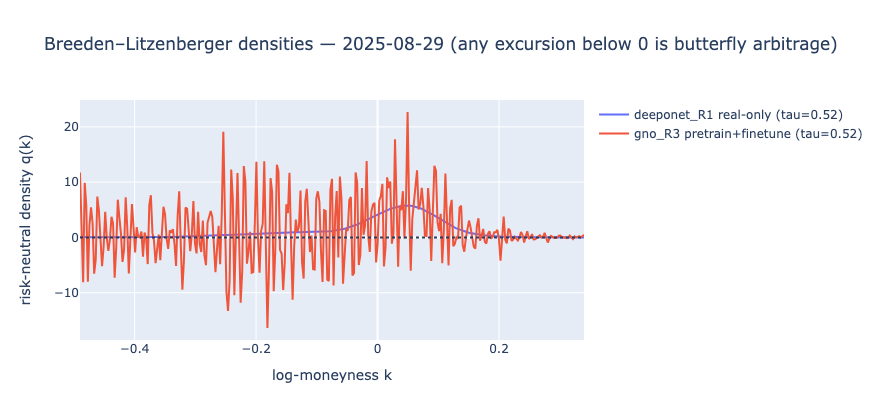
\includegraphics[width=0.95\textwidth]{figures/nb05_c08_1.png}
    \caption{Breeden--Litzenberger densities, 2025-08-29, $\tau=0.52$: the
    DeepONet's density is a smooth nonnegative curve; the GNO's oscillates between $-16$ and
    $+22$ around it---super-unit negative mass invisible to the IV-level fit metric. Source:
    Notebook 05, \S C figure.}
    \label{fig:nb05densities}
\end{figure}

% ============================================================================
\section{F1: a static-arbitrage scanner on bid/ask quotes}\label{sec:scanner}
% ============================================================================

The audits so far interrogate \emph{fitted surfaces}; this section closes the loop by
scanning the \emph{raw quotes}. The scanner asks, per day and per (expiry, type), whether
the quoted bid/ask system already contains \emph{executable} static arbitrage---i.e.\ whether
the market itself violates Proposition~\ref{prop:shape}---priced at the touch (buy at the
offer, sell at the bid), with the same checks at mid prices run alongside: the gap between
the two columns is the bid-ask spread absorbing the ``violations''. It serves two purposes:
it establishes the data-level baseline against which model violation rates must be read (a
model cannot be blamed for reproducing an arbitrage the quotes contain), and it identifies
the stress days on which the ``butterfly binds in stress'' hypothesis of
Section~\ref{sec:realablation} is tested.

\paragraph{Tests.} Per (expiry, type) side, strikes ascending:
\begin{enumerate}[label=(S\arabic*)]
\item \emph{Vertical (monotonicity):} calls must be non-increasing in $K$, puts
non-decreasing; the executable flag is $C^{\mathrm{bid}}(K_{i+1})>C^{\mathrm{ask}}(K_i)$
(sell the spread, collect a positive premium against a nonnegative payoff;
Proposition~\ref{prop:shape}(a), monotone part), and symmetrically for puts.
\item \emph{Butterfly (convexity):} for consecutive strike triples $K_1<K_2<K_3$ with
weights $\lambda_1=(K_3-K_2)/(K_3-K_1)$, $\lambda_3=(K_2-K_1)/(K_3-K_1)$, the executable
flag is $\lambda_1C^{\mathrm{ask}}(K_1)-C^{\mathrm{bid}}(K_2)+\lambda_3C^{\mathrm{ask}}(K_3)<0$
(buy the wings at the ask, sell the body at the bid;
Proposition~\ref{prop:shape}(a), convex part).
\end{enumerate}
Counts are reported per day (absolute and as a share of checks), with the total premium
locked by executable violations in index points, over $250$ days sampled uniformly across
2018--2025, and stored (\texttt{nb05\_static\_arb.parquet}) alongside the per-day model
audit columns so that data-level and model-level rates are directly comparable.

\paragraph{Results.} Over $1{,}926$ trading days the scanner checks roughly $1.22\times10^7$
vertical pairs and $1.21\times10^7$ butterfly triples. At the touch it finds
\textbf{62 executable violations in total}---$6$ vertical and $56$ butterfly---concentrated on
\textbf{$43$ of the $1{,}926$ days} ($2.2\%$), locking a cumulative premium of $18.3$ index
points across eight years: the SPX quote system is, to first order, free of executable static
arbitrage. The mid-price count is larger by orders of magnitude ($2.5\times10^4$ vertical and
$2.6\times10^6$ butterfly flags, at least one on \emph{every} one of the $1{,}926$ days), and
the entire gap between the two columns is the bid--ask spread: the ``violations'' a mid-quote
surface would report are absorbed by the spread and are not transactable. This is the
data-level baseline the model audits must be read against---a model cannot be faulted for a
violation the executable quotes do not contain---and it is the quantitative twin of the
detection-power result of \S\ref{sec:power}: the same market whose residuals sit below the
net-profitability frontier is the market whose quotes admit essentially no executable static
arbitrage. The $43$ flagged days concentrate in the ultra-short bucket, the same bucket where
fitted-SVI violations concentrate (Table~\ref{tab:buckets}), consistent with part of the
short-end difficulty being \emph{in the data} rather than in the smoother.

% ============================================================================
\section{F2: residual relative value---economic significance, not alpha}\label{sec:residual}
% ============================================================================

\paragraph{This is not an arbitrage.} The strategy studied here is \emph{relative value}, not
arbitrage, and the distinction is the one drawn in Section~\ref{sec:twoquestions}. An arbitrage
has a payoff structure guaranteeing no loss in any state, executable at quoted prices. What
follows has no such structure: it ranks options by their residual
$r_i=\sigma^{\mathrm{mkt}}_i-\sigma^{\mathrm{model}}_i$, goes long the cheap tail and short the
rich tail, and profits only if residuals mean-revert on average. It can lose in any given
period. It is a statistical claim about the information content of the residuals, not a claim
about a mispricing that can be locked in. We therefore test economic significance and never
alpha, and we report the result as a comparison between a clean and a deliberately
arbitrage-dirty surface on identical universes with identical costs, rather than as a trading
recommendation.

The next question is whether the surface's \emph{residuals} carry economic information, and
whether arbitrage-dirtiness degrades it. The claim under test is deliberately modest---%
\emph{economic significance}, explicitly not alpha.

\paragraph{Protocol.} Per (day, family): residuals
$r_i=\mathrm{IV}^{\mathrm{mkt}}_i-\mathrm{IV}^{\mathrm{model}}_i$ on \emph{held-out,
in-domain} quotes; matched to $t+h$ by (\texttt{exdate},\,strike). Two layers. \emph{(E)
Information:} $\mathrm{IC}=\mathrm{Spearman}(r_t,-\Delta\mathrm{IV}_{t\to t+1})$ and a
decile spread net of entry half-spreads. \emph{(F2) Backtest:} a \textbf{common universe}
per day (held-out quotes inside \emph{every} model's domain, finite cost, cap
$5\,\vp$---identical names and costs across models, only the surface differs),
bucket-neutral ranking ($\tau$-terciles $\times$ $|k|$-terciles), an \textbf{entry filter}
(trade only quotes mispriced beyond their own half-spread---the F1 bridge), swept over
holding horizons $h\in\{1,3,5,10\}$ and an execution ladder (\emph{touch} = full spread
paid, \emph{half}, \emph{mid} = none: \emph{mid} bounds the market-maker capture of the
signal, \emph{touch} is what a taker pays). First-order vega P\&L, one round trip per
holding period, non-overlapping periods, fit-gated at $5\,\vp$ day RMSE. Costs are real
per-name quote half-spreads converted through Black vega. The thesis link is the
\emph{counterfactual}: the same day smoothed with $\lambda=10$ (clean) and $\lambda=0$
(dirty), same quotes, same universe, same costs.

\paragraph{Information layer (staging: 11 days).} On the controlled synthetic validation
(mean-reverting quote noise by construction) the pipeline behaves as designed: clean-surface
IC $0.712$ against dirty-surface IC $0.455$ on the same day and quotes. On the real staging
days the ICs are small and unstable in sign, as they must be at this sample size (DeepONet
$-0.62$ to $+0.37$ across the ten 2025 days; GNO $\approx0$; SSVI $-0.61$ to $+0.36$), and
the single real clean-vs-dirty day (2018-01-08) is statistically indistinguishable
(IC $0.260$ vs $0.277$): at $n=10$ days this layer is pipeline validation, not evidence.

\begin{table}[htbp]\centering\small
\caption{F2 backtest, mean net P\&L per holding period (\vp), staging sample (deep rows:
one period, 2018-01-08; operator/SSVI rows: the ten 2025-08 days). Sharpe, drawdown and hit
rate are computed and stored (\texttt{nb05\_backtest\_stats.parquet}) but are meaningless at
$n_{\mathrm{periods}}\le10$ and are not tabulated here; the production run populates them.
Source: Notebook 05, \S F2.}
\label{tab:f2}
\begin{tabular}{lcccc@{\qquad}cccc}
\toprule
 & \multicolumn{4}{c}{execution = touch} & \multicolumn{4}{c}{execution = mid} \\
Model & $h{=}1$ & $3$ & $5$ & $10$ & $h{=}1$ & $3$ & $5$ & $10$ \\
\midrule
Deep ($\lambda{=}10$) & $-2.06$ & $-1.36$ & $-1.29$ & $-0.58$ & $+0.08$ & $+0.45$ & $+0.61$ & $+1.12$ \\
Deep ($\lambda{=}0$, dirty) & $-2.10$ & $-1.57$ & $-1.45$ & $-1.23$ & $+0.05$ & $+0.30$ & $+0.59$ & $+0.75$ \\
DeepONet R1 & $-0.74$ & $-0.79$ & $-1.24$ & --- & $-0.05$ & $-0.15$ & $-0.69$ & --- \\
GNO R3 & $-0.67$ & $-0.81$ & $-1.17$ & --- & $-0.06$ & $-0.28$ & $-0.67$ & --- \\
SSVI & $-0.75$ & $-1.09$ & $-1.53$ & $-1.78$ & $+0.01$ & $-0.01$ & $-0.14$ & $-0.09$ \\
\bottomrule
\end{tabular}
\end{table}

Two results survive the small sample. \textbf{(1) Nothing clears the touch.} Every model,
every horizon: net P\&L at the touch is negative---the residual signal, where it exists,
does not pay the spread. This is not a failure of the machinery
(\S\ref{sec:power} validates that an injected signal lights it up); it is a property of the
market, quantified next. \textbf{(2) Clean dominates dirty, cell by cell.} On the matched
counterfactual, the clean surface's P\&L exceeds the dirty one's in \emph{all eight}
(horizon $\times$ execution) cells---at mid, where the residual signal is actually
monetisable by a liquidity provider, $+1.12$ vs $+0.75\,\vp$ at $h=10$---on identical
universes and identical costs.

\begin{finding}[Arbitrage-dirtiness is a signal tax]\label{find:economics}
On matched counterfactuals (same day, quotes, universe, costs), the residual signal computed
against an arbitrage-dirty surface is weaker than against its clean twin: IC $0.455$ vs
$0.712$ on the synthetic validation, and lower net P\&L in $8/8$ backtest cells on the real
staging day. The violation is not only a pricing defect of the surface but a contamination
of everything computed \emph{against} it. (Statistical confirmation at production scale;
the staging sample is a pipeline validation.)
\end{finding}

\begin{figure}[htbp] \centering 
\includegraphics[width=0.95\textwidth]{\detokenize{figures/nb05 F2 cumulative net P&L figure.png}} \caption{Cumulative net P\&L at $h=1$, touch execution, common universe: every family bleeds the spread---the visual of result (1). Source: Notebook 05, \S F2 figure.} \label{fig:nb05f2} \end{figure}

% ============================================================================
\section{G: detection power---the net-profitability frontier of this market}\label{sec:power}
% ============================================================================

F2 measures the signal that \emph{exists}; this section measures the signal this pipeline
and this market \emph{could detect and monetise if it existed}---turning F2's uniformly
negative touch row from an absence of evidence into a measurement of the market.

\paragraph{Protocol.} Take a real day (2025-08-28; universe $1{,}760$ names with real
per-name half-spreads) and inject a synthetic mispricing of amplitude $a$ (vol points,
random sign) into $10\%$ of names, decaying toward the surface with half-life $h$ (trading
days). Run the injected residuals through the \emph{same} F2 machinery (entry filter,
bucket-neutral deciles, real costs) and compute annualised net Sharpe at the touch over the
best holding horizon, over $120$ replications per $(a,h)$ cell. Two calibrations keep the
exercise honest: the observation noise through which the signal must be detected is the
robust dispersion of \emph{actual} residuals ($\sigma_{\mathrm{obs}}=3.92\,\vp$), and the
outcome noise is the robust dispersion of \emph{actual} matched day-over-day IV moves net of
per-expiry common shifts ($\sigma_\varepsilon=0.09\,\vp$/day, idiosyncratic).

\paragraph{Results.} The breakeven frontier at the touch: a mispricing must have amplitude
$\ge3.0\,\vp$ (half-life $\le5$ days) to $\ge5.0\,\vp$ (half-life $8$--$12$ days) to be
net-profitable, best exploited at the longest holding horizon ($10$ days). The pipeline
validation passes: an injected $a=5\,\vp$, $h=12$-day signal produces annualised Sharpe
$18.4$---the machinery detects large persistent signals, so F2's empty real-data result is a
property of the market, not of the code. Against this frontier, the \emph{empirical}
residual distribution of the same day: $98.1\%$ of quotes sit beyond their own half-spread,
but with a median exceedance of only $2.55\,\vp$ and a day-1 residual autocorrelation of
$+0.90$ (half-life $\approx6.9$ trading days)---i.e.\ the empirical point
($2.55\,\vp$, $\sim$7d) sits \emph{below} the $3$--$5\,\vp$ breakeven contour.

\begin{finding}[The spread prices out the residual signal]\label{find:frontier}
On real SPX spreads and measured noise, a residual mispricing must exceed
$\approx3\,\vp$ with multi-day persistence to clear touch costs; the market's empirical
residuals (median exceedance $2.55\,\vp$, half-life $\approx7$d) sit below that frontier.
``No net alpha at the touch'' is thereby a demonstrated property of the market's spread
structure---the quantitative twin of the F1 scan---not an artifact of the pipeline, which
provably detects signals above the frontier.
\end{finding}

\begin{figure}[htbp] \centering 
\includegraphics[width=0.95\textwidth]{\detokenize{figures/nb05 G frontier heatmap.png}} \caption{The detection-power frontier: annualised net Sharpe at the touch as a function of injected amplitude $a$ and half-life $h$; black contour = breakeven. The empirical residual point sits below it. Source: Notebook 05, \S G figure.} \label{fig:nb05g} \end{figure}

\section{Path-dependence: what an arbitrage-dirty surface actually costs}\label{sec:barrier}
% ============================================================================

Every object priced so far is \emph{terminal} or \emph{static}: held-out repricing
(\S\ref{sec:localvol}), Breeden--Litzenberger densities (\S\ref{sec:densities}), the
variance-swap rate (\S\ref{sec:vix}). Each depends on the surface only through a
\emph{marginal} distribution at a single maturity---and that is precisely where an
arbitrage-dirty surface looks least damaged, because the fitting objective is itself a
marginal-distribution objective: a surface that reproduces the vanilla prices reproduces the
marginals almost by construction. The Dupire local volatility, by contrast, is the
\emph{instantaneous dynamics}, not a marginal object; a defect in $g$ between the collocation
nodes perturbs the diffusion coefficient along every path that visits that region. The
economic consequence must therefore be sought where this chapter has not yet looked: in a
path-dependent payoff.

We close that gap with one instrument---a discretely monitored down-and-out call---under a
controlled experiment whose ground truth is \emph{a third model}, related to neither candidate
surface. The design isolates the one quantity of interest (the cost of the arbitrage defect)
from the two effects that would otherwise confound it (finite-difference numerics and the
local-vol-versus-stochastic-vol model gap).

\paragraph{An independent ground truth.} Circularity is the obvious trap: if the paths that
judge two desks are generated from the \emph{clean} surface's own local volatility, the clean
desk wins by construction. We therefore generate truth from a Heston model
($v_0{=}0.035$, $\kappa{=}1.8$, $\theta{=}0.045$, $\xi{=}0.65$, $\rho{=}-0.72$), which is
neither surface. Vanilla quotes come from its characteristic function (exact to quadrature);
barrier truth and hedging paths come from Monte Carlo on the same parameters, the MC engine
first validated against the characteristic-function pricer on vanillas
($<0.1\,\vp$ IV error). Heston is a genuine martingale model, so the synthetic market it
defines is itself arbitrage-free---there is no arbitrage in the quotes to find---yet it is not
a local-volatility model, so its Dupire projection reproduces every marginal but not the joint
law across monitoring dates. That last gap is real and irreducible; we measure it separately
(below) so it is never mistaken for the defect effect.

\paragraph{Two surfaces, matched on vanillas by construction.} The clean surface is a
GJ-certified SSVI prior fitted to the synthetic quotes. The dirty surface is the same object
times a node-aligned defect, $w_{\mathrm{dirty}}=w_{\mathrm{clean}}\,(1+a\,\psi)$ with
$\psi(k,\tau)=\sin(2\pi k/\Delta k)\,\mathrm{env}(\tau)$ and $\Delta k$ the quoted log-strike
spacing. Because $\sin(2\pi k_j/\Delta k)=0$ at every quoted strike $k_j$, the defect is
\emph{exactly zero on the entire quote lattice}: the vanilla RMSE is unchanged to machine
precision for any amplitude. This is the collocation blind spot of Finding~\ref{find:blindspot}
in its purest form---a surface perfectly controlled \emph{at} the nodes and uncontrolled
\emph{between} them---and $a$ is a \emph{dose}, not a fitted quantity, so sweeping it traces a
dose--response curve on which the real operator surfaces can be placed. The dirtiness enters
through curvature: for the ripple $w_{kk}\sim a\,w\,(2\pi/\Delta k)^2$, so with $\Delta k=0.04$
a dose of $a\approx10^{-3}$ suffices to drive $g<0$ while leaving the fit invariant
(Table~\ref{tab:barrieraudit}).

\begin{table}[htbp]\centering\small
\caption{Node-aligned defect: identical vanilla fit, growing arbitrage violation. The RMSE
column is invariant to machine precision (the defect vanishes on the quote lattice); the
repair rate is the share of the vega-trusted local-vol grid where $\sigma_{\mathrm{loc}}^2$ is
invalid. Source: Notebook 06, \S B3 (\texttt{nb06\_surface\_audit.parquet}).}
\label{tab:barrieraudit}
\begin{tabular}{lccccc}
\toprule
Surface & Dose $a$ & Vanilla RMSE (\vp) & $\min g$ & LV repair (core) & LV repair (all) \\
\midrule
clean          & $0$       & $0.348605$ & $+0.316$ & $0.0\%$    & $0.0\%$    \\
ripple         & $0.0002$  & $0.348605$ & $+0.148$ & $0.0\%$    & $0.0\%$    \\
ripple         & $0.0005$  & $0.348605$ & $-0.126$ & $0.98\%$   & $0.98\%$   \\
ripple         & $0.001$   & $0.348605$ & $-0.583$ & $6.16\%$   & $6.25\%$   \\
ripple         & $0.002$   & $0.348605$ & $-1.496$ & $11.42\%$  & $11.80\%$  \\
ripple         & $0.004$   & $0.348605$ & $-3.322$ & $15.81\%$  & $16.69\%$  \\
\bottomrule
\end{tabular}
\end{table}

\paragraph{The error budget.} A single mispricing number is worthless unless the reader knows
what else could produce it. Three gaps sit between the Heston truth and a barrier price
computed from a fitted surface, and Notebook~06 \S B4 measures them separately. \emph{(1)
Numerical:} the barrier-aligned Crank--Nicolson PDE against local-vol Monte Carlo under the
\emph{same} local volatility---pure discretisation, which must sit inside MC noise. It does:
across the four barriers the PDE--MC gap is $\{+1.35,-0.15,-0.59,-0.65\}$ MC standard errors,
i.e.\ statistically zero. \emph{(2) Model-class:} local volatility against Heston, both
reproducing the same marginals---$0.48$--$1.45\%$ of price, the irreducible
Dupire-versus-stochastic-vol difference and the scale against which any defect effect must be
judged. \emph{(3) Defect:} dirty against clean, both fitted to the same quotes with the same
RMSE---the quantity of interest, isolated. Two further validations pass: the Dupire round trip
(a vanilla repriced through the extracted local volatility) closes to $-0.27$\,bp,
certifying that extraction and PDE are mutually consistent on the very vanilla the surface was
fitted to; and the vanilla PDE matches Black to $-0.06$\,bp, the discrete barrier
matches the Broadie--Glasserman--Kou continuity-corrected closed form to $\le0.35$\,bp.

\paragraph{One numerical lesson, worth stating.} Computing $g$ by finite differences on an
implied-variance grid extracted from \emph{exact} Heston prices produced $\min g=-4.13$ and a
$9.2\%$ repair rate---on a surface that is arbitrage-free by construction. The violations were
entirely an artefact: in the deep wings at short maturity the Black vega collapses, the
price-to-implied-vol inversion is ill-conditioned, and the second $k$-difference amplifies the
residual without bound. Restricting the audit to a \emph{vega-trusted core}
($\varphi(d_1)>10^{-3}$) and extending the local variance flat in $k$ outside it, the same
surface reads $\min g=+0.35$ and a repair rate of exactly zero. The lesson generalises
Finding~\ref{find:blindspot} to differentiation once more: any reported violation rate on a
finite-difference grid is a joint statement about the surface \emph{and} the conditioning of
the extraction, and the two must be separated before a violation is attributed to the model.
Every repair rate in this section is reported on the vega-trusted core.

\subsection{The dose--response: identical fit, divergent exotic price}

\begin{table}[htbp]\centering\small
\caption{Down-and-out call ($K{=}F$, monitored barrier $B$), synthetic experiment. Price
impact and hedging error are stated relative to the clean surface, which fits the vanilla
market identically ($0.3486\,\vp$) at every dose. $\Delta V$ = model mispricing; hedging
$\mathrm{sd}$ and $5\%$ tail are the dispersion and left tail of the \emph{paired} per-path
P\&L difference (\S\ref{sec:barrierhedge}), as a percentage of the clean premium. Source:
Notebook 06, \S B5--B6 (\texttt{nb06\_barrier\_sweep}, \texttt{nb06\_hedging}).}
\label{tab:barriersweep}
\begin{tabular}{lccccc}
\toprule
Dose $a$ & LV repair & $\Delta V$ ($B{=}0.90$) & $\Delta V$ ($B{=}0.85$) & Hedge sd ($B{=}0.90$) & Hedge 5\% tail ($B{=}0.90$) \\
\midrule
$0.0002$ & $0.0\%$    & $+0.03\%$ & $+0.02\%$ & $\phantom{0}0.5\%$  & $-0.3\%$  \\
$0.0005$ & $0.98\%$   & $-0.06\%$ & $+0.06\%$ & $\phantom{0}1.3\%$  & $-1.0\%$  \\
$0.001$  & $6.16\%$   & $+0.31\%$ & $+0.13\%$ & $\phantom{0}2.6\%$  & $-2.4\%$  \\
$0.002$  & $11.42\%$  & $-2.37\%$ & $-2.37\%$ & $11.2\%$            & $-14.7\%$ \\
$0.004$  & $15.81\%$  & $-3.29\%$ & $-2.37\%$ & $22.3\%$            & $-30.1\%$ \\
\bottomrule
\end{tabular}
\end{table}

Table~\ref{tab:barriersweep} is the point of the notebook, and it carries a sharper message
than a monotone dose--response would. The damage tracks the \emph{repair rate}---the
arbitrage violation---not the perturbation amplitude. While the dose is large enough to move
the surface but too small to break no-arbitrage (repair $\approx0$, $a\le0.0002$), the barrier
price is unmoved and the sign of $\Delta V$ is ambiguous. The moment the defect forces
local-variance repair (repair $\gtrsim11\%$, $a\ge0.002$), $\Delta V$ becomes material,
$-2.4\%$ to $-3.3\%$ of premium, on a surface whose vanilla RMSE has not moved in its fifth
decimal. It is not moving the surface that costs money; it is \emph{breaking the no-arbitrage
structure}. The headline figure~\ref{fig:nb06sweep} plots this directly: vanilla RMSE on the
horizontal axis, barrier mispricing on the vertical---the clean and dirty surfaces occupy the
same vertical line and spread without bound.

\thfig{figures/nb06_fig01.pdf}{0.95}{The defect the vanilla fit cannot see. Left column: the
clean surface's Dupire local volatility $\sigma_{\mathrm{loc}}$ (top) and Durrleman
$g$ (bottom), everywhere valid. Right column: the dirtiest node-aligned surface at the same
vanilla RMSE to machine precision---$\sigma_{\mathrm{loc}}$ with repaired cells in red (top)
and $g$ turning negative between the quoted strikes (bottom). The defect lives strictly in the
inter-node gaps the calibration objective never samples. Source: Notebook 06, \S B3.}{fig:nb06audit}

\thfig{figures/nb06_fig03.pdf}{0.95}{The collocation blind spot priced. Left: barrier
mispricing against vanilla RMSE---the horizontal axis (fit) barely moves while the vertical
axis (exotic price error) does not stop. Right: the same against the local-vol repair rate,
showing that the damage is a function of the arbitrage violation, not of the fit. Source:
Notebook 06, \S B5.}{fig:nb06sweep}

\subsection{Delta hedging: wrong Greeks, not discrete-hedging noise}\label{sec:barrierhedge}

Mispricing is half the cost. A desk that sells the barrier and hedges it with the wrong delta
bleeds P\&L over the life of the trade even if it happened to sell at the right price. Both
desks sell at the \emph{same} entry price (the clean surface's) and hedge on the \emph{same}
Heston truth paths at the same monitoring dates, each with its own delta. The naive comparison
of two independently computed P\&L standard deviations is dominated by the common
discrete-hedging noise of a barrier---the clean desk's own P\&L has standard deviation
$\approx0.029$, half the premium---so we take the \emph{per-path difference}
$\delta\Pi=\sum_j(\Delta_j^{\mathrm{dirty}}-\Delta_j^{\mathrm{clean}})(S_{j+1}-S_j)$, which
cancels the common term exactly and leaves a pure ``wrong Greeks'' P\&L estimated to high
precision. Its dispersion and $5\%$ tail are the model-risk numbers of
Table~\ref{tab:barriersweep}. At the largest dose the hedging error reaches $22\%$ of the
premium in standard deviation and $-30\%$ in the $5\%$ tail. One structural detail is worth
noting: the hedging error becomes material \emph{before} the price does---already
$1$--$4\%$ at repair $6\%$, where $\Delta V$ is still sub-$1\%$---because the delta is a
\emph{derivative} of the surface and therefore more sensitive to fine-scale defect than the
price, which is an integral. The wrong Greeks bite first.

\thfig{figures/nb06_fig04.pdf}{0.9}{Model-risk hedging error from wrong Greeks: standard
deviation of the \emph{paired} per-path P\&L difference (dirty minus clean desk, same Heston
paths, common discrete-hedging noise removed), as a percentage of the clean premium, against
the defect dose. The vanilla RMSE is invariant along the horizontal axis. Source: Notebook 06,
\S B6.}{fig:nb06hedge}

\subsection{The same measurement on the real operator surfaces}\label{sec:barrierreal}

The synthetic experiment supplies a controlled dose and an independent truth at the price of a
synthetic market. Notebook~06 \S B8 applies the identical barrier machinery to the actual
exported NB03/NB04 surfaces, with two disciplines: the barrier and strike must sit strictly
inside each pack's exported box (extrapolated local volatility is not the surface), and a
\emph{fit-parity gate} governs which pairs may be compared. No ground truth exists here, so
the reported quantities are differences between models, not errors; read together with the
calibrated synthetic curve, they place the real surfaces on the dose--response.

\begin{table}[htbp]\centering\small
\caption{Real down-and-out call ($B{=}0.90$), per operator family, averaged over staging days
inside each pack's domain. The graph operator has the \emph{best} vanilla fit and a barrier
price collapsed by $60\%$, on a local-vol surface half of which is invalid. The prior-embedded
DeepONet---the response to the operator critique---has the best fit \emph{and} zero repair
\emph{and} a sound price. Source: Notebook 06, \S B8 (\texttt{nb06\_real\_barrier.parquet}).}
\label{tab:barrierreal}
\begin{tabular}{lcccc}
\toprule
Family & Vanilla RMSE (\vp) & LV repair (core) & Barrier price & Days \\
\midrule
DeepONet-prior R1 (real-only)     & $\mathbf{1.11}$ & $0.0\%$          & $0.0557$          & 4 \\
GNO R3 (pretrain+finetune)        & $1.51$          & $\mathbf{52.2\%}$ & $\mathbf{0.0223}$ & 4 \\
DeepONet R3 (pretrain+finetune)   & $2.69$          & $0.09\%$         & $0.0595$          & 4 \\
Deep smoother ($\lambda{=}10$)    & $2.44$          & $0.0\%$          & $0.0576^{\ast}$   & 20 \\
Deep smoother ($\lambda{=}0$)     & $2.01$          & $0.0\%$          & $0.0561^{\ast}$   & 4 \\
\bottomrule
\end{tabular}\\[2pt]
{\footnotesize $^{\ast}$ deep-smoother price at the nearest reported barrier; both
$\lambda$ settings are arbitrage-clean in the liquid zone (\S\ref{sec:realablation}), so the
$\lambda{=}0$ counterfactual is not the dirty surface \emph{on real data}---the GNO is.\\
The GNO's $52\%$ local-volatility repair rate and its $21.2\%$ butterfly-audit rate
(Table~\ref{tab:opaudit}) are \emph{distinct} quantities and are not in tension: the former
counts every cell of the $\sigma_{\mathrm{loc}}^2=\partial_\tau w/g$ grid that is invalid
(both signs of failure, plus the calendar numerator), the latter only butterfly violations of
$g$ as a fraction of the audit area. A surface can be butterfly-violating on a fifth of its
area and yet, through the ratio, produce invalid local variance on half of it.}
\end{table}

Table~\ref{tab:barrierreal} is the chapter's sharpest single exhibit, and it is the
Table~\ref{tab:unified} inversion made monetary. The GNO has the \emph{best or near-best
vanilla fit in the study} ($1.51\,\vp$, better than either deep-smoother setting and than
DeepONet~R3) and prices the barrier at $0.0223$ against $\approx0.056$--$0.060$ for every
other family: a $60\%$ collapse, driven by a local-volatility surface invalid on $52\%$ of its
grid. A desk selecting on IV-RMSE buys the GNO and prices this exotic at $40\%$ of its value.
The resolution sits one row above: the prior-embedded DeepONet, the constructive answer to the
operator critique, achieves the \emph{best} fit in the table \emph{with} zero repair \emph{and}
a barrier price in line with the clean families. The prior does not cost accuracy; it removes
the downstream damage. This is \emph{replicate $\to$ diagnose $\to$ repair} closed on an
exotic, in dollars.

Two caveats are stated rather than hidden. First, the fit-parity gate: the GNO fits
\emph{better} than the clean references, so a naive ``it prices badly because it fits badly''
is unavailable---the gate \emph{fails} for GNO-vs-clean precisely because the GNO is the more
accurate surface, which strengthens the reading rather than weakening it (the price gap cannot
be a fit-quality gap). Second, on real data the $\lambda{=}0$ ablation does not produce a dirty
surface in the liquid zone (repair $0\%$, Table~\ref{tab:localvol}); the penalty is not what
protects the deep smoother there. On real SPX the arbitrage-dirty object is the graph operator,
and it breaks on its own.

\begin{finding}[Arbitrage violations are model risk, not foregone alpha]\label{find:exotic}
A surface can fit the vanilla market identically to a certified arbitrage-free surface
(Table~\ref{tab:barrieraudit}) and still misprice a path-dependent product by
$2$--$3\%$ of premium while injecting hedging error of tens of percent
(Table~\ref{tab:barriersweep}); on real data the study's most accurate operator misprices a
down-and-out call by $60\%$ off a half-invalid local-vol surface (Table~\ref{tab:barrierreal}).
The cost of a collocation blind spot is not a free lunch the market failed to remove
(Findings~\ref{find:economics},~\ref{find:frontier})---it is model risk realised on every
exotic derived from the surface, and it is removed, at no cost in fit, by a certified prior.
\end{finding}

% ============================================================================
\section{VIX replication: external ground truth for the wings}\label{sec:vix}
% ============================================================================

The 30-day variance-swap rate integrates the whole smile:
$\sigma_{VS}^2T=2\int\tilde q(k)e^{-k}\dd k$ with $\tilde q$ the normalized OTM Black price
at $(k,w(k,T))$, total variance interpolated linearly in $\tau$ to $T=30/365$, the integral
taken over the \emph{common $k$-strip of the day's models} so families at different export
ranges are comparable. Compared daily to the published VIX (CBOE \texttt{VIX\_History},
$2{,}178$ days 2018--2026) it is an \emph{external} ground truth that scores exactly what
hold-out RMSE cannot: the wings. Machinery self-tested on flat Black--Scholes ($0.1997$ vs
$0.200$, truncation-limited).

\begin{table}[htbp]\centering\small
\caption{VIX replication on the staging days (model variance-swap minus published VIX, \vp,
on the day's common $k$-strip). Source: Notebook 05, \S D.}
\label{tab:vix}
\begin{tabular}{lcccc}
\toprule
Model & mean err (\vp) & mean $|$err$|$ (\vp) & $k$-strip & days \\
\midrule
Deep ($\lambda{=}10$), 2018-01-08 & $+1.28$ & 1.28 & 2.47 & 1 \\
DeepONet R1, 2025-08 & $-1.61$ & 1.61 & 0.83 & 10 \\
GNO R3, 2025-08 & $+0.51$ & 0.51 & 0.83 & 10 \\
\bottomrule
\end{tabular}
\end{table}

Table~\ref{tab:vix} must be read with the sign convention, and it delivers one more
inversion. On the narrow common strip ($k$-width $0.83$) a truncated integral of an
\emph{accurate} surface must sit \emph{below} the VIX: the DeepONet's systematic
$-1.6\,\vp$ combines this truncation deficit with its coarse wings. The GNO's
$+0.5\,\vp$---nominally the best $|$err$|$---is therefore \emph{not} superior wings: a
surplus at identical truncation means the surface manufactures spurious wing variance, and
$\approx2\,\vp$ of the GNO's variance-swap value is its own oscillation
(\S\ref{sec:densities}) masquerading as smile. A naive $|$err$|$ ranking would crown the
GNO here exactly as IV-RMSE does in Table~\ref{tab:opaudit}: the third instance of the same
inversion, and the reason the cross-model ordering is only meaningful \emph{jointly} with
the audit columns.

% ============================================================================
\section{Unified evaluation and discussion}\label{sec:unified}
% ============================================================================

\subsection{One table, four questions}

\begin{table}[htbp]\centering
\caption{The unified view. Fit is hold-out IV RMSE under the shared $\mathrm{crc32}$
protocol (NB02: 8-day staging; NB03: staging days; NB04: 386 chronological out-of-sample
days). Audit columns are \emph{material} rates on grids independent of any penalty grid.
Downstream columns from this chapter (staging days). Cost is per new day on CPU. Entries
marked $^\dagger$ are staging-scale and replaced by the production run at submission.}
\label{tab:unified}
\resizebox{\textwidth}{!}{%
\begin{tabular}{lcccccc}
\toprule
 & Fit, hold-out (\vp) & Guarantee & Material viol.\ (audit) & LV repair & Density neg.\ mass & Cost / day \\
\midrule
SVI (per slice)      & $0.64^\dagger$ & none (audited ex post) & 12\% of slices$^\dagger$ & n/a (no $\partial_\tau w$) & slice-level $g<0$ & $\sim$1\,s \\
SSVI (certified)     & $1.91^\dagger$ & \textbf{theorem} (Thm.~\ref{lem:range}) & 0\% & 0\% & 0\% & $\sim$1\,s \\
Deep ($\lambda{=}10$)& $1.7$--$1.8^\dagger$ & soft + certified prior & 0\% (staging) & 0\% & 0\% & 80--100\,s \\
DeepONet (best)      & $\approx2.3$ & soft, train days only & $\le0.97\%$ & 0.3--0.6\% & $\approx0$ & $<$1\,ms \\
GNO (best)           & $\approx1.6$ & soft, train days only & \textbf{21.2\% bfly} & \textbf{49--52\%} & up to \textbf{230\%} & 40--400\,ms \\
\bottomrule
\end{tabular}}
\end{table}

Table~\ref{tab:unified} answers the four questions the thesis poses of any smoother.
\emph{How well does it fit?} Per-slice SVI still leads on staging accuracy; the deep
smoother and the graph operator sit inside the SVI--SSVI window, the operator at amortised
cost. \emph{What does it guarantee, and on what set?} Only SSVI (and hence the deep
smoother's prior) carries a theorem; the neural penalties guarantee their sampling
sets---and, for operators, only their training days. \emph{What does a failure cost?} This
chapter's columns: the graph operator's fit advantage is bought with a local-variance
surface half invalid, densities with up to $230\%$ negative mass, $8\,\vp$/day
local-vol instability, $\approx2\,\vp$ of spurious variance-swap value, and---on a
path-dependent down-and-out call priced off that half-invalid surface---a $60\%$ collapse in
the exotic's price relative to a clean family that fits the vanillas \emph{worse}
(\S\ref{sec:barrier}, Table~\ref{tab:barrierreal}). \emph{What does
it cost to run?} The operator's four-orders-of-magnitude latency advantage is real and
quantified---the honest statement of its value proposition is \emph{speed at the price of
un-transported constraints}, not accuracy.

\subsection{Threats to validity}

\textbf{Scale.} NB02/NB03 numbers are staging-scale (marked $^\dagger$); the production run
(\texttt{LIMIT\_DATES=None}, \texttt{EXPORT\_ALL}, $\sim$30\,h CPU parallelised by year;
operator retraining on GPU with raised epochs) replaces them without code changes. The
operator accuracy/audit results (386 out-of-sample days) are already at scale; the
downstream staging set is $11$ days. \textbf{Under-training.} Operator epoch budgets were
CPU-bound; validation curves were still descending, so accuracy entries are lower
bounds---but nothing in the blind-spot mechanism improves with epochs: the penalty is
already minimised on its grid. \textbf{FD asymmetry.} Operator packs carry FD-reconstructed
$(g,\partial_\tau w)$; the reconstruction is validated to $1.2\times10^{-4}$ on smooth
references, an order below materiality, and the exact-autodiff deep-smoother packs provide
the control. \textbf{Selection.} Stress days were chosen \emph{ex ante} from the NB02
audit; the stress test is gated; the invariance study is gated; the F2 backtest is
fit-gated; the $\lambda=0$ in-sample anomaly of Section~\ref{sec:realablation} is flagged
as an optimisation artefact and excluded from claims. \textbf{Residual economics.} The
information layer at $n\le10$ days is pipeline validation; the clean-vs-dirty dominance
($8/8$ cells) and the detection frontier are staging results whose statistical confirmation
is the production run's job---and the frontier result (Finding~\ref{find:frontier})
carries its own internal validation (the injected-signal PASS).

\subsection{What we would tell a desk}

(i)~Never read a soft-constraint model's own violation report; demand the node-vs-audit
pair and the material rate. (ii)~If a certified parametric prior is available, use it
multiplicatively: it does the protective work and the corrector buys accuracy on top
(Tables~\ref{tab:ablation},~\ref{tab:localvol}). (iii)~If an operator's speed is needed,
treat its output as a \emph{proposal} and project it (e.g.\ one certified-prior corrector
step, or the Section-\ref{sec:parametric} repairs) before any Greek or density leaves
it---and never score it by MC repricing or variance-swap error alone, both of which launder
the violations (\S\ref{sec:localvol}, \S\ref{sec:vix}). (iv)~Score smoothers on repair
rate, density mass and day-over-day stability, not IV RMSE alone: the ranking inverts three
separate times between those columns. (v)~Do not expect smoothing residuals to pay the
touch on SPX: the breakeven frontier sits at $3$--$5\,\vp$ and the market's residuals live
below it (Finding~\ref{find:frontier}); their value is in marking and market-making
(mid-execution capture), where surface cleanliness is measurably worth
$+0.4\,\vp$ per 10-day period on the staging counterfactual.
(vi)~The place the cleanliness is not optional is exotics: a surface indistinguishable from a
certified one on the vanilla objective can misprice a barrier by $60\%$ and mis-hedge it by
tens of percent of premium (\S\ref{sec:barrier}), and the wrong Greeks bite before the wrong
price does---so project the surface \emph{before} it reaches any path-dependent book, not after
the P\&L appears.